\begin{frame}{The global hackathon: 2022}
  \begin{columns}[c,onlytextwidth]
    \column{.44\textwidth}
      \small
      \NTXPoint{October 29--30, 2022}{Free, global online participation with local chapter hosting.}
      \NTXPoint{Brain-age prediction from EEG}{Child Mind Institute's Healthy Brain Network (HBN) dataset.}
      \NTXPoint{A shared challenge platform}{Paris-Saclay's CodaLab; Sylvain Chevallier's MNE / scikit-learn starting kit.}
    \column{.52\textwidth}
      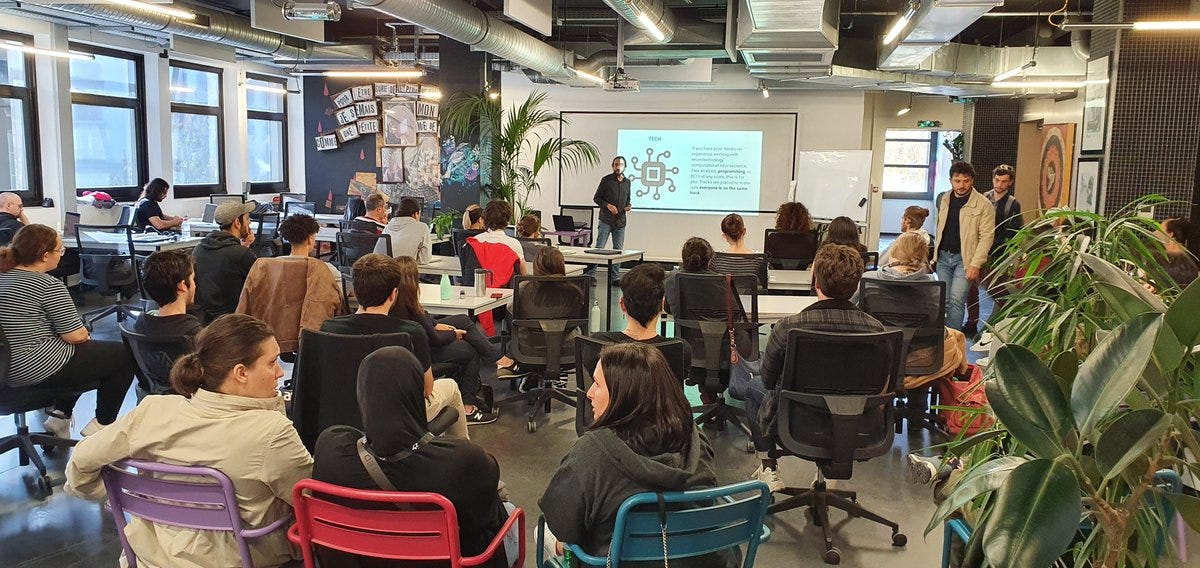
\includegraphics[width=\linewidth,height=44mm,keepaspectratio]{assets/chapters/paris-global-hackathon-2022.jpg}
      \par\smallskip{\scriptsize Briefing session in Paris\par}
  \end{columns}
  {\tiny\color{NTXMuted}Sources: \href{https://tailor-network.eu/brain-age-prediction-challenge/}{TAILOR}; \href{https://codalab.lisn.upsaclay.fr/competitions/8336}{CodaLab}; \href{https://gist.github.com/sylvchev/206f93acd7393ab3b955602eba42d427}{starting kit}; HBN: Morgan Hough; photo: NTX Content Lab / Firas Safieddine\par}
  \note{The photo is captioned Briefing session in Paris in the official Content Lab retrospective, published December 3, 2022. The program advertised five locations; the later retrospective reports six including New York. Do not confuse the advertised list with a final attendance audit.}
  \note{[33:45--34:45] Historical context, approximately one minute. Morgan identifies the data task as brain-age prediction using Child Mind Institute Healthy Brain Network EEG and confirms CodaLab as the platform. TAILOR's November 16, 2022 announcement verifies the brain-age task and Paris-Saclay CodaLab competition 8336; it gives November 4--22 as the challenge window, distinct from the October 29--30 hackathon. Sylvain's October 30 starting kit uses MNE, scikit-learn pipelines, PCA, and ridge regression. This was an EEG machine-learning challenge, not a deep-learning-only contest or a clinically validated brain-age diagnostic. The Content Lab retrospective credits Inria, TAILOR, Universite Paris-Saclay, and LISN. Do not confuse this with the separate RAMP/OpenBHB MRI brain-age challenge. Earlier hosting details remain in the source archive.}
\end{frame}

\begin{frame}{The global hackathon: 2023}
  \begin{columns}[c,onlytextwidth]
    \column{.44\textwidth}
      \small
      \NTXPoint{December 2--3, 2023}{Second annual global event: free and hybrid.}
      \NTXPoint{Eight advertised locations}{Paris, Vienna, Zurich, Delhi, Kharagpur, Bras\'{i}lia, Buenos Aires, London.}
      \NTXPoint{Four tracks}{Hardware; data; design and strategy; new ethics track.}
    \column{.52\textwidth}
      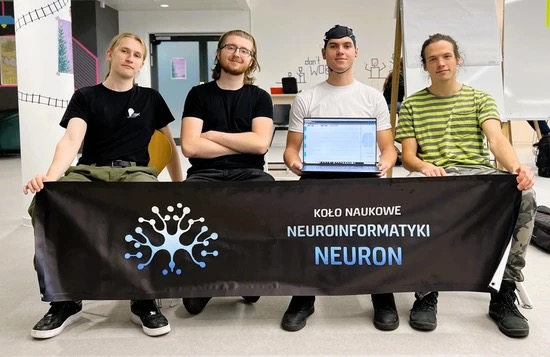
\includegraphics[width=\linewidth,height=42mm,keepaspectratio]{assets/chapters/vienna-global-hackathon-2023.jpg}
      \par\smallskip{\scriptsize Neuron club team, Vienna\newline ``Bore No More'' --- second in software\par}
  \end{columns}
  \smallskip{\scriptsize Historically coordinated with \'Ecole 42 across multiple cities.\par}
  {\tiny\color{NTXMuted}Sources: \href{https://neurotechx.com/hackathon2023/}{2023 program}; photo: \href{https://wit.pwr.edu.pl/en/news/students-from-the-neuron-club-successful-in-ntx-hackathon-163.html}{Wroc\l{}aw University of Science and Technology}; coordination: Morgan Hough\par}
  \note{[34:45--35:45] Historical context, approximately one minute. The 2023 program lists eight host cities and adds ethics as a fourth track; advertised locations do not establish attendance or growth. Morgan confirms historical multi-city coordination with Ecole 42; both official event pages display its sponsor logo, but no specific campus list or exclusive organizing role is inferred. The university recap identifies Neuron students Pawel Dzikiewicz, Tomasz Koralewski, Jakub Ner, and Adam Pawlowski presenting Bore No More in Vienna and placing second in software. This is the global hackathon, not the separate student club competition. No generalizable classifier-performance or clinical claim is made. Photo provenance is recorded in assets/chapters/event-photo-sources.md.}
\end{frame}
